\documentclass[11pt,letterpaper]{article}
\usepackage[margin=2cm,includefoot]{geometry}
\usepackage[spanish]{babel}
\usepackage{graphicx}

%%%%% Lenguajes
\newcommand{\pl}{\textsc{Prolog}}
\newcommand{\hsk}{\textsc{Haskell}}
\newcommand{\coql}{\textsc{Coq}}

%%%%%
\renewcommand{\H}{\mathcal{H}}
\newcommand{\B}{\mathcal{B}}
\renewcommand{\S}{\mathcal{S}}
\newcommand{\R}{\mathcal{R}}
\newcommand{\T}{\mathcal{T}}

%%%%% Simbolos logicos
\newcommand{\true}{\mathop{\mathsf{true}}}
\newcommand{\E}{\ensuremath{\exists}}

\newcommand{\dy}{\vee}
\newcommand{\cj}{\wedge}
\newcommand{\imp}{\rightarrow}
\newcommand{\Imp}{\Rightarrow}
\renewcommand{\iff}{\leftrightarrow}
\newcommand{\Iff}{\Leftrightarrow}
\newcommand{\syss}{\leftrightarrow}

\newcommand{\fa}{\forall}
\newcommand{\ex}{\exists}

\newcommand{\G}{\Gamma}
\newcommand{\D}{\Delta}
\newcommand{\Lb}{\Lambda}
\newcommand{\Om}{\Omega}

\newcommand{\lb}{\lambda}
\newcommand{\al}{\alpha}
\newcommand{\ga}{\gamma}

\newcommand{\bool}{\mathsf{Bool}}
\newcommand{\propo}{\ensuremath{\mathsf{PROP}}}
\newcommand{\atom}{\ensuremath{\mathsf{ATOM}}}
\newcommand{\term}{\ensuremath{\mathsf{TERM}}}
\newcommand{\form}{\ensuremath{\mathsf{FORM}}}

\newcommand{\vars}{\ensuremath{\mathsf{Var}}}
\newcommand{\Var}{\ensuremath{\mathsf{Var}}}

\newcommand{\vphi}{\varphi}
\newcommand{\vp}{\varphi}


%%%%% Sustitucion
\newcommand{\sust}[2]{[#1 := #2]}

%alpha equivalencia 
\newcommand{\aeq}{\;\;\sim_\al\;\;}

%%%%% Programacion logica
\newcommand{\pmi}{\leftarrow}

\newcommand{\impp}{\ensuremath{\,\text{:-}\,}\,}
\newcommand{\meta}{\ensuremath{\;\text{?-}\;}}
\newcommand{\si}{\sigma}

\renewcommand{\P}{\mathbb{P}}


%%%%% Razonamiento ecuacional

% \renewcommand{\P}{\mathcal{P}}

\newcommand{\J}{\mathcal{J}}
\newcommand{\hip}[2]{#1:#2}

\newcommand{\eqdef}{=_{def}}

\newcommand{\pf}[2]{#1\vdash#2}
\newcommand{\bk}[2]{#1\vdash_{\bkc}#2}
\newcommand{\bkd}[2]{#1\vdash_{\bkdc}#2}
\newcommand{\tcp}[2]{#1\vdash_{C}#2} %??

\newcommand{\bkc}{\mathcal{B}}
\newcommand{\bkdc}{\mathcal{B}^{\textsc{Dem}}}

%%%%% Deduccion natural
\newcommand{\dn}{\mathsf{DN}}
\newcommand{\dnC}{\mathsf{DN_C}}
\newcommand{\dnM}{\mathsf{DN_M}}
\newcommand{\dnp}{\mathsf{DN_p}}
\newcommand{\dnm}{\mathsf{DN_p^M}}
\newcommand{\dnc}{\mathsf{DN_p^C}}

\newcommand{\Dnm}{\mathsf{DN_m}}
\newcommand{\Dni}{\mathsf{DN_i}}
\newcommand{\Dnc}{\mathsf{DN_c}}
%\newcommand{\dnp}{\mathsf{DN}}
% \renewcommand{\vp}{A}
% \renewcommand{\psi}{B}
% \renewcommand{\chi}{C}


%%%%% Resolucion binaria
\newcommand{\cv}{\Box}
\newcommand{\sat}{\textsf{SAT}}
\newcommand{\modsrch}{\models_?}



%%%%% Simbolos matematicos

\newcommand{\inc}{\subseteq}
\newcommand{\iso}{\ensuremath{\cong}}
\newcommand{\union}{\ensuremath{\cup}}
\newcommand{\morinyec}{\ensuremath{\precapprox}}
\newcommand{\nin}{\ensuremath{\notin}}
\newcommand{\niso}{\ensuremath{\not \cong}}

\newcommand{\restr}[2]{#1\!\!\boldsymbol{\restriction}\!#2}

\newcommand{\vacio}{\varnothing}
\newcommand{\ol}[1]{\overline{#1}}

\newcommand{\supc}{\supseteq}
\newcommand{\limo}{\mathop{\mathpzc{Lim}}}
\newcommand{\ord}{\mathsf{OR}}


\newcommand{\vx}{\vec{x}}
\newcommand{\vy}{\vec{y}}
\newcommand{\vz}{\vec{z}}
\newcommand{\vt}{\vec{t}}
\newcommand{\vf}{\vec{f}}

%%%%% Curry-Howard
% \newcommand{\true}{\mathsf{true}}
\newcommand{\false}{\mathsf{false}}
\newcommand{\ifte}[3]{\mathsf{if\;}#1\mathsf{\; then\;}#2\mathsf{\;
    else\;}#3}
\newcommand{\iszero}{\mathop{\mathsf{iszero}}}
%\newcommand{\suc}{\mathop{\mathsf{succ}}}
\newcommand{\pred}{\mathop{\mathsf{pred}}}
\newcommand{\suc}{\mathop{{\sf suc}}}
\newcommand{\no}{\mathop{{\sf not}}}
\newcommand{\fun}{\mathop{{\sf  fun}}}
\newcommand{\inl}{\mathop{{\sf inl }}}
\newcommand{\inr}{\mathop{{\sf inr }}}
\newcommand{\nat}{\mathsf{Nat}}
\newcommand{\Tf}{\mathsf{T}}

\newcommand{\Lp}{{\tt fst}}
\newcommand{\Rp}{{\tt snd}}

\newcommand{\ejp}{\mathop{\mathtt{ejp}}}
\newcommand{\ej}{\mathop{\mathtt{ej}}}
\newcommand{\comp}{\mathop{\mathtt{comp}}}
\newcommand{\eval}{\mathop{\mathtt{eval}}}
\newcommand{\ap}{\mathop{\mathtt{+\!\!\!+}}}


%%%%% Identificadores

\newcommand{\A}{\mathcal{A}}
% \newcommand{\Q}{\ensuremath{\mathbb{Q}}}
% \newcommand{\Z}{\ensuremath{\mathbb{Z}}}
% \newcommand{\N}{\ensuremath{\mathbb{N}}}
% \newcommand{\R}{\ensuremath{\mathbb{R}}}

\newcommand{\F}{\mathcal{F}}
\newcommand{\Ge}{\mathcal{G}}
\newcommand{\Pe}{\mathcal{P}}
\newcommand{\I}{\mathcal{I}}
\newcommand{\C}{\mathcal{C}}
\newcommand{\K}{\mathcal{K}}
\newcommand{\Kb}{\mathbb{K}}
\newcommand{\Eb}{\mathbb{E}}
\newcommand{\Ebs}{\mathbb{E}^\star}
\newcommand{\Ob}{\mathbb{O}}
\newcommand{\Ib}{\mathbb{I}}
\newcommand{\kb}{\bbkappa}
\newcommand{\M}{\mathcal{M}}
\newcommand{\Nc}{\mathcal{N}}
%\newcommand{\E}{\mathcal{E}}
%\newcommand{\R}{\mathcal{R}}
%\newcommand{\Q}{\mathcal{Q}}
\newcommand{\Sc}{\mathcal{S}}
\newcommand{\Sf}{\mathsf{\Sigma}}
\renewcommand{\S}{\mathbb{\Sigma}}
\newcommand{\Te}{\mathcal{T}}
\newcommand{\Rb}{\mathbb{R}}
\newcommand{\Qb}{\mathbb{Q}}
\newcommand{\Kbb}{\mathbb{K}}
% \newcommand{\T}{\mathbb{\Theta}}
\renewcommand{\L}{\mathcal{L}}


\newcommand{\Db}{\mathbb{D}}
\newcommand{\Fb}{\mathbb{F}}
\newcommand{\De}{\mathcal{D}}

\newcommand{\mg}{\mathbb{m}}

\newcommand{\cg}{\mathbb{C}}
\newcommand{\dg}{\mathbb{D}}
\newcommand{\jg}{\mathbb{J}}
\newcommand{\Ha}{\mathcal{H}}
%\newcommand{\A}{\mathcal{A}}
\newcommand{\sg}{\mathbb{S}}

\newcommand{\Mg}{\mathbb{M}}
\newcommand{\Bg}{\mathbb{B}}
\newcommand{\Lg}{\mathbb{L}}
\newcommand{\Tg}{\mathbb{T}}

% \newcommand{\B}{\mathbb{B}}
\newcommand{\N}{\mathbb{N}}

\newcommand{\W}{\mathcal{W}}

\newcommand{\Bc}{\mathcal{B}}
\newcommand{\Df}{\mathfrak{D}}
\newcommand{\Dc}{\mathcal{D}}
%\newcommand{\Tc}{\mathcal{T}}
\newcommand{\Mf}{\mathfrak{M}}

\newcommand{\Sg}{\mathbb{S}}

\newcommand{\Tsf}{\mathsf{T}}


%\newcommand{\id}{\mathsf{Id}}

%\newcommand{\uc}{\mathcal{U}}
%\newcommand{\Ic}{\mathcal{I}}
%\newcommand{\pc}{\mathcal{P}}
%\newcommand{\qc}{\mathcal{Q}}
%\newcommand{\mc}{\mathcal{M}}


%%%%% Cosmetics
\newcommand{\la}{\left\langle}
\newcommand{\ra}{\right\rangle}

\newcommand{\inds}[1]{\index[simb]{#1}}

\newcommand{\ida}{$\Rightarrow \; )$ }
\newcommand{\regr}{$\Leftarrow \; )$ }
% \newcommand{\done}{\ensuremath{\checkmark}}

\newcommand{\espc}{\vspace*{.3cm}}
\newcommand{\pt}[1]{\langle #1 \rangle}

\newcommand{\bc}{\begin{center}}
\newcommand{\ec}{\end{center}}
\newcommand{\be}{\begin{enumerate}}
\newcommand{\ee}{\end{enumerate}}
\newcommand{\bi}{\begin{itemize}}
\newcommand{\ei}{\end{itemize}}
 \newcommand{\beq}{\begin{equation}}
 \newcommand{\eeq}{\end{equation}}
 \newcommand{\beqs}{\begin{equation*}}
 \newcommand{\eeqs}{\end{equation*}}
\newcommand{\ba}{\begin{array}}
\newcommand{\ea}{\end{array}}

\newcommand{\bej}{\begin{ejercs}}
\newcommand{\eej}{\end{ejercs}}

\newcommand{\ggf}{{\tt gg\,}}

\newenvironment{prueba}{\vspace{-5mm}\noindent\textbf{Demostraci\'on}\\}{
\noindent$\blacksquare$\\}

\def\stackunder#1#2{\mathrel{\mathop{#2}\limits_{#1}}}


%\newtheorem{lema}{Lema}
\newtheorem{teorema}{Teorema}
\newtheorem{corolario}{Corolario}
\newtheorem{definicion}{Definición}
\newtheorem{proposicion}{Proposición}


\newtheorem{theorem}{Teorema}
\newcommand{\teo}[1]{\begin{theorem} #1 \end{theorem}}
\newtheorem{proposition}{Proposici\'on}
\newcommand{\prop}[1]{\begin{proposition} #1 \end{proposition}}
\newtheorem{definition}{Definici\'on}
\newcommand{\defin}[1]{\begin{definition} #1 \end{definition}}
\newtheorem{corollary}{Corolario}
\newcommand{\cor}[1]{\begin{corollary} #1 \end{corollary}}
\newtheorem{lemma}{Lema}
\newcommand{\lema}[1]{\begin{lemma} #1 \end{lemma}}
% \newcommand{\dem}[1]{\begin{proof} #1 \end{proof}}

% \newcommand{\proof}{ \vspace*{-15pt} \hfill\\\noindent\textbf{\textit{
% Demostraci\'on. }}}

\DeclareMathAlphabet{\mathpzc}{OT1}{pzc}{m}{it}

%\newcommand{\case}{\mathsf{case}}
%\renewcommand\labelitemi{$\circ$}
%%\newcommand{\qed}{\hfill$\mathbb{Qed}$}
% \newcommand{\qed}{\hfill$\mathsf{\boldsymbol{\dashv}}$}

\newtheorem{eje}{Ejemplo}
\newcommand{\ejem}[1]{\begin{eje}\normalfont #1 \end{eje}}

\newcommand{\hint}[1]{\textit{\textbf{Sugerencia:} #1}}


\newcounter{EjempCtr}[section]
\newenvironment{enumrom}{\renewcommand{\theenumi}{\roman{enumi}}
\renewcommand{\theenumii}{\roman{enumii}}
\renewcommand{\theenumiii}{\roman{enumiii}}
\renewcommand{\theenumiv}{\roman{enumiv}}
\begin{enumerate}}{\end{enumerate}}
\newenvironment{Ejemplo}
        {\stepcounter{EjempCtr}%
        \begin{description}\item[Ejemplo \thesection.\arabic{EjempCtr}]}%
        {\end{description}}
\newenvironment{demostr}{{\em Demostración:}
        \begin{quotation}}{\end{quotation}}

\newcommand{\beje}{\begin{Ejemplo}}
\newcommand{\eeje}{\end{Ejemplo}}




%%%%% Notas
% \newcommand{\doubt}{\Red{{\LARGE {\sf ??}}}}
% 
% \newcommand{\coment}[1]{\hfill\\ \Big[{\bf Comentario Privado:} #1\Big]}
% \newcommand{\preg}[1]{\hfill\\ \BrickRed{{\bf Pregunta:} #1}}
% \newcommand{\conjet}[1]{\hfill\\ \OliveGreen{{\bf Conjecura:} #1}}
% 
% \newcommand{\pendiente}{\BrickRed{{\sc Pendiente}}}
% \newcommand{\verifpendiente}{\BrickRed{{\sc Verificación pendiente}}}

% \newcommand{\sketch}{\Red{{\sc sketch}}}
   
%%=================================================================================
%%%%% Y estos para que sirven???
% \newcommand{\tog}{\makebox[7mm][l]}
% \newcommand{\toge}{\makebox[11mm][l]}
% \newcommand{\toget}{\makebox[13mm][l]}
% \newcommand{\togeth}{\makebox[14mm][l]}
% \newcommand{\togethe}{\makebox[15mm][l]}
% \newcommand{\together}{\makebox[17mm][l]}

% \renewcommand\contentsname{\'Indice}
%\renewcommand\chaptername{Cap\'itulo}
% \renewcommand\indexname{\'Indice}
% 
%%\newcommand{\qed}{\hfill$\mathbb{Qed}$}
%\newcommand{\qed}{\hfill$\mathsf{\boldsymbol{\dashv}}$}
%\renewcommand{\qed}{\hfill$\boldsymbol{\dashv}$}
%\newcommand{\qed}{\hfill$\mathbb{Qed}$}


% \newcommand{\Ejercicios}{\section*{Ejercicios}}
% \newenvironment{manitas}{%
%       \renewcommand{\labelitemi}{\ding{44}}%
%       \vspace{-0.5cm}%
%       \begin{itemize}%
%       
% \setlength{\itemsep}{0pt}\setlength{\parsep}{0pt}\setlength{\topsep}{0pt}%
%       }{\end{itemize}}
% \newenvironment{malitos}{%
%       \renewcommand{\labelitemi}%
%             {\raisebox{1.5ex}{\makebox[0.3cm][l]{\begin{rotate}{-90}%
%             \ding{43}\end{rotate}}}}%
%       \vspace{-0.5cm}%
%       \begin{itemize}%
%       
% \setlength{\itemsep}{0pt}\setlength{\parsep}{0pt}\setlength{\topsep}{0pt}%
%       }{\end{itemize}}
% \newenvironment{ejercs}{
%      \renewcommand{\labelenumi}{\thesection.\theenumi.-}
%      \renewcommand{\labelenumii}{\theenumii)}
%      \begin{enumerate}}
%      {\end{enumerate}}

%\newenvironment{leterize}{%
%        \renewcommand{\theenumi}{\alph{enumi}}
%        \begin{enumerate}}{\end{enumerate}}

%\newenvironment{manitas}{%
%      \renewcommand{\labelitemi}{\ding{44}}%
%      \vspace{-0.5cm}%
%      \begin{itemize}%
%      \setlength{\itemsep}{0pt}\setlength{\parsep}{0pt}\setlength{\topsep}{0pt}%
%      }{\end{itemize}}


%\renewcommand{\qed}{\qedsymbol{$\mathbf{\dashv}$}}

\graphicspath{ {images/} }

\usepackage{hyperref}
\usepackage{csquotes}
\usepackage{multicol}

\usepackage{qtree}

\usepackage{amsmath}
\usepackage{amsthm}
\usepackage{amssymb}
\usepackage{listings}


\title{Tarea Examen 2}
\author{Diego Méndez Medina}
\date{}


\begin{document}

\ttfamily
\maketitle
\rmfamily

\begin{enumerate}

  % 01
\item {\bf 1.5 pts}  Considera la siguiente fórmula:
  \[
  \forall y \forall x \Big(\exists w (Txa \land Rw) \imp Pyu 
  \lor Txy \Big)
  \]


  \begin{itemize}
    % a
  \item Proporciona el \'arbol de sintaxis abstracta que representa la misma 
    f\'ormula.

    \Tree[.$\forall y$ [
        .$\forall x$ [
          .$\rightarrow$ [
            [.$\exists w$ [.$\land$ [.$T$ [.$x$ ][.$a$ ]][.$R$ [.$w$ ]]]]
            [.$\lor$ [.$P$ [.$y$ ][.$u$ ]][.$T$ [.$x$ ][.$y$ ]]]]]]]

    
    % b 
  \item Indica el alcance de cada cuantificador.

    \begin{itemize}
    \item El alcance de $\forall y$ es:
      $$\forall x \Big(\exists w (Txa \land Rw) \imp Pyu \lor Txy \Big)$$

    \item El alcance de $\forall x$ es :
      $$\exists w(Txa \land Rw) \imp Pyu \lor Txy$$

    \item El alcance de $\exists w$ es:
      $$Txa \land Rw$$
      
    \end{itemize}
    
    % c
  \item Da el conjunto de predicados y funciones, indicando su aridad.

    No existen funciones.

    Los predicados con su ariedad son: $T^2, R^1$ y $P^2$.
    
    % d
  \item Indica el conjunto de variables libres y ligadas.

    \begin{align*}
      Ligadas &= \{x, y, w\}\\
      Libres &= \{u\} 
    \end{align*}
    
    % e
  \item Aplica la sustitución 
    $\sigma = [w,x,u := z,\;fw,\;fy]$ 
    Debes mostrar los renombres de variables o las f\'ormulas $\alpha$
    equivalentes que utilices en el proceso.

    Primera observación:
    $\sigma = [w:= z,\, x:= fw,\, u := fy]$

    \begin{align*}
      \forall y \forall x \Big(\exists w (Txa \land Rw) \imp Pyu 
      \lor Txy \Big)[w:= z,\, x:= fw,\, u := fy] &\equiv_\alpha\\
      \forall p \forall q \Big(\exists r (Tqa \land Rr) \imp Ppu 
      \lor Tqp \Big)[w:= z,\, x:= fw,\, u := fy] = \\
      \forall p \forall q \Big(\exists
      r (Tqa \land Rr)[w:= z,\, x:= fw,\, u := fy] \imp (Ppu 
      \lor Tqp)[w:= z,\, x:= fw,\, u := fy] \Big) = \\
      \forall p \forall q \Big(\exists r (Tqa \land Rr) \imp Ppfy 
        \lor Tqp \Big)
    \end{align*}
    
  \end{itemize}

  \bigskip
  % 02
\item {\bf 0.5 pts}  ¿Cuál es la simbolización más adecuada para la 
  afirmación
  \textit{Nadie está totalmente loco si un doctor lo ayuda}\\
  Donde: $Dx$ se lee como \textit{$x$ es doctor}; $Tx$ se lee como \textit{$x$ 
    está totalmente loco}; $Axy$ se lee como \textit{$x$ ayuda a $y$}
  \begin{enumerate}
    \item $\fa x (\ex y(Dy \land  Axy) \land  \lnot Tx)$
    \item $ \ex x \ex y (Dx \land  Ayx \to  \lnot Tx)$
    \item $\fa x (\ex y(Dy \land  Ayx) \to  Tx)$
    \item $\boxed{\fa x (Tx \to  \lnot \ex y( Dy \land  Ayx))}$
  \end{enumerate}
  
  \bigskip
  % 03
\item {\bf 0.5 pts}  ¿A qué equivale la negación lógica de:
  \textit{Todos los amigos de son enemigos de Ana} ?
  \begin{enumerate}
  \item  Algún amigo de Juan es amigo de Ana.
  \item  Ningún amigo de Juan es amigo de Ana.
  \item  Algún enemigo de Ana no es amigo de Juan.
  \item  \fbox{Algún amigo de Juan no es enemigo de Ana.}
  \end{enumerate}
  \bigskip

  % 04
\item{\bf 2 pts}  {\it Hunting the Wumpus} Este juego se desarrolla en un tablero de dos dimensiones como el que se muestra en la siguiente figura:
  
  \begin{center}
    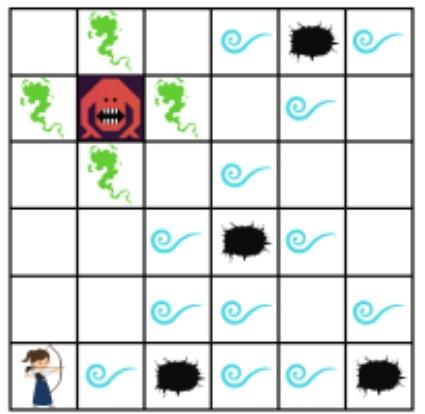
\includegraphics[scale=.3]{wumpus1}
  \end{center}
  
  El objetivo del juego es que el aventurero mate al Wunpus y tome el tesoro, para lo cuál solo dispone de una flecha.
  
  Cada casilla del tablero  puede estar vacía o contener alguno de los siguientes elementos:
  \bi
\item El aventurero
\item El Wumpus
\item Un pozo
\item Viento
\item Olor a pies
\item Una combinación de viento y olor a pies
  \ei
  
  La especificación del juego es la siguiente:
  \bi
\item El aventurero inicia el juego en la casilla inferior izquierda, marcada con la coordenada $(0,0)$
\item El Wumpus no puede estar en una casilla ocupada por un pozo.
\item El jugador no conoce el tablero, es decir, desconoce en donde se encuentra cada elemento. Solo puede {\bf percibir} el contenido de la casilla en la que se encuentra y recuerda las casillas por las que paso.
\item Según las percepciones del aventurero en cada casilla puede inferir información nueva:
  \bi
\item Si percibe olor a pies, puede inferir que el Wumpus está en una casilla adyacente.
\item Si percibe viento, puede inferir que hay un pozo en una casilla adyacente.
\item Si percibe una combinación de olor a pies y viento, puede inferir que hay tanto un pozo como el Wumpus en las casillas adyacentes.
\item Si percibe un grito, infiere que el Wumpus ha muerto.
  \ei 
\item Cada viento corresponde a un único pozo. 
\item Las únicas casillas consideradas adyacentes son las que colindan al norte, sur, oriente y poniente, mas no las diagonales.
  \ei
  El aventurero puede realizar una de las siguientes acciones:
  \bi
\item Moverse a una de las casillas adyacentes (no puede caminar en diagonal).
\item Disparar al norte, sur, oriente o poniente (no en diagonal) y el alcance de la flecha es hasta donde termina la fila o la columna sobre la que disparo en la dirección del disparo. el Wumpus muere si es alcanzado por una flecha y emite un grito.
\item Asesinar al Wumpus. En este caso el juego termina y el aventurero gana.
\item Si entra a la casilla en donde se encuentra el Wumpus y este sigue con vida, lo devorará vivo. en este caso el juego termina y el aventurero pierde.
\item Si entra a una casilla con un pozo, caerá al vacío y morirá. En este caso el juego termina y el aventurero pierde.
  \ei
  
  Puedes jugar unas partidas del juego para entenderlo mejor en el siguiente enlace \url{https://osric.com/wumpus/}
  Formaliza las siguientes reglas del juego con los siguientes predicados:

  \bi
\item $Axy$ el aventurero está en la casilla $(x,y)$.
\item $Wxy$ el Wumpus está en la casilla $(x,y)$.
\item $Pxy$ hay un pozo en la casilla $(x,y)$.
\item $Vxy$ hay viento en la casilla $(x,y)$.
\item $Oxy$ hay olor a pies en la casilla $(x,y)$.
\item $Lxy$ la casilla $(x,y)$ está libre.
  \ei
  \begin{enumerate}
    % a
  \item Si hay olor a pies en una casilla el Wumpus se encuentra en alguna de las casillas adyacentes.

    $$Oxy \rightarrow (W(x,y+1)\lor W(x,y-1)\lor W(x+1,y)\lor W(x-1,y))$$

    Asumimos que si $x/y\, +/-\, 1$ no figura en el tablero no causa
    problema.

    % b
  \item Si hay viento en una casilla entonces hay un pozo en alguna de las casillas adyacentes.

    $$ Vxy \rightarrow (P(x,y+1)\lor P(x,y-1)\lor P(x+1,y)\lor P(x-1,y))$$

    Asumimos que si $x/y\, +/-\, 1$ no figura en el tablero no causa
    problema.
    % c
  \item Si la casilla $(x,y)$ está libre, entonces no está el Wumpus ni hay pozos en las casillas adyacentes.

    \begin{align*}
      Lxy \rightarrow (&\neg P(x,y+1)\land\neg P(x,y-1)\land\neg P(x+1,y)
    \land\neg P(x-1,y)\land\\
    &\neg W(x,y+1)\land\neg W(x,y-1)\land\neg W(x+1,y)
    \land\neg W(x-1,y))
    \end{align*}

    Asumimos que si $x/y\, +/-\, 1$ no figura en el tablero no causa
    problema.

    % d
  \item Una casilla está libre si no hay olor a pies, viento, pozo o el Wumpus en ella.

    $$Lxy\leftrightarrow (\neg Oxy\land \neg Vxy\land \neg Pxy\land \neg Wxy)$$
    % e
  \item formaliza cada uno de los movimientos permitidos del aventurero, es decir, las reglas correspondientes a su desplazamiento.

    Hacemos uso de un nuevo predicado:

    $Dxy$ = El aventurero puede desplazarse a la casilla $(x, y)$

    $$Axy \rightarrow (D(x+1, y)\lor D(x-1, y)\lor D(x, y+1)\lor
    D(x, y-1))$$
    
    De nuevo asumimos que si $x/y\, +/-\, 1$ no figura en el tablero no causa
    problema.
  \end{enumerate}

  Formaliza el siguiente tablero y prueba que en la celda $(0,2)$ hay un pozo.
  
  \begin{center}
    
\includegraphics[scale=0.3]{wumpus2}
  \end{center}

  Formalización del estado del tablero:
  \begin{align*}
    A11 \land V01\land V12\land O13\land L00\land L01\land L02 \land L12
    \land L22
  \end{align*}

  Probando que en (0,2) hay un pozo:
  \begin{align*}
    &V01 & &\text{Por estado del tablero} & &(1)\\
    &V12 & &\text{Por estado del tablero} & &(2)\\
    &A11 & &\text{Por estado del tablero} & &(3)\\
    &L00 & &\text{Por estado del tablero} & &(4)\\
    &L22 & &\text{Por estado del tablero} & &(5)\\
    &V01 \rightarrow P00\lor P02 \lor P11 & &\text{Regla del juego y estado}
    & &(6)\\
    &L00 \rightarrow \neg P00 & &\text{Regla del juego y estado}  & &(7)\\
    &\neg P00 & &\text{Por $(7)$ y $(4)$} & &(8)\\
    &V01 \rightarrow P02 \lor P11 & &\text{Por $(6)$ y $(8)$}  & &(9)\\
    &A11 \rightarrow L11 & &\text{Sigue vivo y estado} & &(10)\\
    &V01 \rightarrow P02 & &\text{Por $(9)$ y $(10)$}  & &(11)\\
    &P02 & &\text{Por $(11)$ y $(1)$} & &\blacksquare
  \end{align*}

  También es facíl ver que Wumpus está en la casilla $(4,1)$. 
  % 05 
\item {\bf 1.5 pts} Decide si los siguientes argumentos lógicos son correctos o exhibe un contraejemplo mostrando paso a paso la prueba o la construcción del contraejemplo.
  \begin{itemize}
    % a)
  \item $\exists x(Ax\land\lnot Bx),\exists x(Bx\land\lnot Ax) / \therefore \forall x (Ax\lor Bx)$
    
    Mostraremos un contraejemplo. Sea:
    
    \begin{align*}
      Ax &=_{def} x \text{ es un número primo}\\
      Bx &=_{def} x \text{ es un número impar}
    \end{align*}

    Y $\mathcal{M} = <M, \mathcal{I}>$ tal que:
    
    \begin{align*}
      M &= \{2,3,4,9\} &\implies \Int(A) &= \{3,2\}\\
      & & \Int(B) &= \{3, 9\}\\
    \end{align*}

    Entonces:
    \begin{align*}
      \Int(A2) &= 1 & &\text{Pues } 2 \in A^\Int & &(1)\\
      \Int(\neg B2) &= 1 & &\text{Pues } 2 \notin B^\Int & &(2)\\
      \Int_{[x/2]}(Ax \land\lnot Bx) &= 1 & &\text{Por $(1)$ y $(2)$} & &(3)\\
      \Int(\exists x(Ax\land\lnot Bx)) &= 1 & &\text{Por $(3)$} & &(4)\\
      \Int(B9) &= 1 & &\text{Pues } 9 \in B^\Int & &(5)\\
      \Int(\neg A9) &= 1 & &\text{Pues } 9 \notin A^\Int & &(6)\\
      \Int_{[x/9]}(Bx \land\lnot Ax) &= 1 & &\text{Por $(5)$ y $(6)$} & &(7)\\
      \Int(\exists x(Bx\land\lnot Ax)) &= 1 & &\text{Por }(7) & &(8)\\
    \end{align*}
    De tal forma que las premisas son correctas en $\m$, pero veremos
    que la conclusión no lo es:

    \begin{align*}
      \Int(A4) &= 0 & &\text{Pues } 4\notin A^\Int & &(9)\\
      \Int(B4) &= 0 & &\text{Pues } 4\notin B^\Int & &(10)\\
      \Int_{[x/4]}(Ax\lor Bx) &= 0 & &\text{Por $(9)$ y $(10)$} & &(11)\\
      \Int(\forall x (Ax\lor Bx)) &= 0 & &\text{Por $(11)$}
    \end{align*}

    Mostramos un contraejemplo donde el modelo de las premisas no lo son
    para la conclusión, entonces el argumento no es correcto.
    \bigskip
    % b)
  \item $\exists x(Ax\to (Bx\lor Cx)),\exists xAx / \therefore \exists x Bx$

    Mostraremos otro contraejemplo. Sea:

    \begin{align*}
      Ax &=_{def} x \text{ es multiplo de cuatro}\\
      Bx &=_{def} x \text{ es cuatro}\\
      Cx &=_{def} x \text{ es mayor o igual que ocho}
    \end{align*}

    y $\m = < M, \Int>$, tal que:

    \begin{align*}
      M &= \{8,12,16\} &\implies B^\Int &= \emptyset\\
      & & A^\Int &= \{8, 12, 16\}\\
      & & C^\Int &= \{8, 12, 16\}\\
    \end{align*}

    Así:
    \begin{align*}
      \Int(A8) &= 1 & &\text{Pues } 8 \in A^\Int & &(1)\\
      \Int_{[x/8]}(Ax) &= 1 & &\text{Por } (1) & &(2)\\
      \Int(\exists x\,Ax) &= 1 & &\text{Por } (2) & &(3)\\
      \Int(C8) &= 1 & &\text{Pues } 8 \in C^\Int & &(4)\\
      \Int_{[x/8]}(Cx) &= 1 & &\text{Por } (4) & &(5)\\
      \Int(\exists x\,(Bx\lor Cx)) &= 1 & &\text{Por } (5) & &(6)\\
      \Int(\exists x\,(Ax\rightarrow Bx\lor Cx)) &= 1 & &\text{Por $(2)$ y
        $(5)$}  & &(7)\\
    \end{align*}

    Entonces las premisas son verdaderas en $\m$, pero la conclusión
    no lo es, pues $B^\Int$ no tiene elementos.
    
  \end{itemize}

  \newpage
\item {\bf 1 pto}   Realiza las siguientes sustituciones indicando los pasos m\'as 
  importantes, en particular aquellos donde se usa la $\alpha$-equivalencia:
  \bi
\item $\Big(\forall x (Ruvw \lor Px) \imp \exists y \big(Pfy \lor 
  Ryxa\big)\Big) [u,v , w, x, y:=fa, gx, y, hu, fa]$

  \begin{align*}
    \Big(\forall x (Ruvw \lor Px) \imp \exists y \big(Pfy \lor 
    Ryxa\big)\Big) [u,v , w, x, y:=fa, gx, y, hu, fa] &\equiv_\alpha\\
    \Big(\forall z (Ruvw \lor Pz) \imp \exists s \big(Pfs \lor 
    Rsxa\big)\Big) [u,v , w, x, y:=fa, gx, y, hu, fa] &= \\
    \forall z (Ruvw \lor Pz)[u,v , w, x, y:=fa, gx, y, hu, fa] \imp
    \exists s \big(Pfs \lor 
    Rsxa\big) [u,v , w, x, y:=fa, gx, y, hu, fa] &= \\
    \forall z (Rfagxy \lor Pz)\imp
    \exists s \big(Pfs \lor 
    Rshua\big) &= 
  \end{align*}
  % b)
\item $\forall x (Sx \imp (\neg Qyx \lor \exists z Rzx) [y:=z] \land \forall y Qxy) [z:=x]$

  \begin{align*}
    \forall x (Sx \imp (\neg Qyx \lor \exists z Rzx) [y:=z]
    \land \forall y Qxy) [z:=x] &\equiv_\alpha \\
    \forall x (Sx \imp (\neg Qyx \lor \exists u Rux) [y:=z]
    \land \forall y Qxy) [z:=x] &=\\
    \forall x (Sx \imp (\neg Qzx \lor \exists u Rux)
    \land \forall y Qxy) [z:=x] &\equiv_\alpha\\
    \forall v (Sv \imp (\neg Qzv \lor \exists u Ruv)
    \land \forall y Qvy) [z:=x] &=\\
    \forall v (Sv  [z:=x]\imp (\neg Qzv \lor \exists u Ruv) [z:=x]
    \land \forall y Qvy  [z:=x]) &=\\
    \forall v (Sv \imp (\neg Qxv \lor \exists u Ruv)
    \land \forall y Qvy)
  \end{align*}
  
  % c)
\item $\big(\forall v\exists y Svyz\lor\exists z Pfvgyz\big)
  [w:=fu,u:=hyz, y:=b]$ en donde $f^{(1)},g^{(1)}$
  \begin{align*}
    \big(\forall v\exists y Svyz\lor\exists z Pfvgyz\big)
    [w:=fu,u:=hyz, y:=b]&\equiv_\alpha \\
    \big(\forall v\exists p Svpz\lor\exists x Pfvgyx\big)
    [w:=fu,u:=hyz, y:=b]&= \\
    \forall v\exists p Svpz[w:=fu,u:=hyz, y:=b]\lor\exists
    x Pfvgyx[w:=fu,u:=hyz, y:=b]&= \\
    \forall v\exists p Svpz\lor\exists
    x Pfvgyx[y:=b]&= \\
    \forall v\exists p Svpz\lor\exists
    x Pfvgbx\\
  \end{align*}
  \ei

  \bigskip
\item {\bf 2 pts} Sea $M=\{1,3,5,15\}$ e $\mathcal{I}$ la función de interpretación en $M$ que interpreta los siguientes predicados como se indica:
  \bi 
\item $Ex$: $x$ es par.
\item $Mxy$: $x$ es múltiplo de $y$.
\item $Lxy$: $x$ es menor que $y$.
  \ei

  Verifica si se cumple lo siguiente o en caso contrario da un contraejemplo:

  \begin{enumerate}
  \item $\models\exists y Ey\lor\forall x\lnot Ex$

    Sea $\sigma$ una intepretación de las variablas, dado $|\m|$ solo hay
    un caso:
    \begin{align*}
      I_\sigma(E1) &= 0 & I_\sigma(E3) &= 0 \\
      I_\sigma(E5) &= 0 & I_\sigma(E15) &= 0 \\
    \end{align*}

    Entonces $\Int_\sigma[x/m](\neg Ex)$ para toda $m\in M$. Como $\sigma$ es
    arbitraria, concluimos $\models\exists y Ey\lor\forall x\lnot Ex$.

    % b)
  \item $\models\forall x\forall y(Lxy\to\lnot Lyx)$

    Para cualquier $\sigma$ estado de las variables y $m\in|\m|$ocurre:
    \begin{align*}
      \Int_\alpha(Lmm) &= 0 &\implies \Int_\alpha(\neg Lmm) &= 1\\
      & & \Int_\alpha(Lmm\to\lnot Lmm) &= 1
    \end{align*}

    Sean $n,m\in|\m|$ tales que $n \neq m$, hay dos casos:
    
    \begin{align*}
      \text{Caso }1&:\\
      \Int_\alpha(Lnm) &= 1 & \implies n &< m\\
      & & \Int_\alpha(Lmn) &= 0\\
      & & \Int_\alpha(\neg Lmn) &= 1\\
      &\implies \Int_\alpha(Lnm \rightarrow \neg Lmn) = 1\\
      % 2ndo
      \text{Caso }2&:\\
      \Int_\alpha(Lnm) &= 0 & \implies n &> m\\
      & & \Int_\alpha(Lmn) &= 1\\
      & & \Int_\alpha(\neg Lmn) &= 0\\
      &\implies \Int_\alpha(Lnm \rightarrow \neg Lmn) = 1
    \end{align*}

    Para los tres casos la implicación sigue siendo verdad, entonces
    $\models\forall x\forall y(Lxy\to\lnot Lyx)$.
    
    % c)
  \item $\models\forall x\exists y Lxy\land\forall x\exists y Mxy$

    Contrajemplo:

    Sea $\sigma$ una interptretación de las variables cualesquiera,
    afuerza occure:
    \begin{align*}
      \Int_\alpha(L(15,1)) &= 0 & \Int_\alpha(L(15,3)) &= 0\\
      \Int_\alpha(L(15,5)) &= 0 & \Int_\alpha(L(15,15)) &= 0
    \end{align*}

    Entonces $\Int_\sigma(\exists yL(15, y)) = 0$. Así
    $\not\models\forall x\exists y Lxy\land\forall x\exists y Mxy$
    
    % d)
  \item $\models\forall x(Ex\to Mxa)\to \lnot\exists x Lxa$ en donde $\mathcal{I}(a)= 1$

    Sea $\sigma$ una interpretación de las variables cualesquiera.
    
    Ninguna $m\in|\m|$ es par, entonces $\Int_\sigma(\forall x Ex) = 0$. Así:
    $$ \Int_\sigma(\forall x Ex\to Mxa) = 1$$

    Falta ver que $\Int_\sigma(\lnot\exists x Lxa)$ sea verdadero.

    \begin{align*}
      \lnot\exists x Lxa &\equiv \forall x \lnot Lxa
    \end{align*}

    \begin{align*}
      \Int(L(1,a)) = \Int(L(1,1)) &= 0 & \Int(L(3,a)) = \Int(L(3,1))&= 0\\
      \Int(L(5,a)) = \Int(L(5,1)) &= 0 & \Int(L(15,a)) = \Int(L(15,1))&= 0
    \end{align*}
  \end{enumerate}

  Entonces $\Int_\sigma(\forall x \lnot Lxa) = 1$. Concluimos
  $\models\forall x(Ex\to Mxa)\to \lnot\exists x Lxa$, donde $\mathcal{I}(a)= 1$
  % 08
\item {\bf 1 pts} 
  Decide si los siguientes conjuntos son unificables mediante el algoritmo de 
  Martelli-Montanari, haciendo explícito el proceso de composición de
  sustituciones para calcular el \textbf{umg} final en cada caso.
  \begin{itemize}
    % a
  \item $W=\{Paxfgy,\; Pzfzfw\}$ con $P^{(3)},f^{(1)},g^{(1)}$.

    \begin{align*}
      \{Paxfgy = Pzfzfw\}& & &\text{Entrada}\\
      \{a = z,\, x=fz,\, fgy = fw\}& & &\text{DESC}\\
      \{z = a,\, x=fz,\, fgy = fw\}& & &\text{SWAP}\\
      \{x=fa,\, fgy = fw\}& & &\text{SUST}[z:=a]\\
      \{x=fa,\, fw = fgy\}& & &\text{SWAP}\\
      \{x=fa,\, w = gy\}& & &\text{DESC}\\
      \{x=fa\}& & &\text{SUST}[w:=gy]\\
      \emptyset& & &\text{SUST}[x=fa]\\
    \end{align*}

    El unificador es:
    \begin{align*}
      \mu &= [z:=a][w:=gy][x:=fa]\\
      &= [z:=a,\,w:=gy,\,x:=fa]
    \end{align*}

    Comprobación:

    \begin{align*}
      \{Paxfgy,\; Pzfzfw\}[z:=a,\,w:=gy,\,x:=fa] &= \\
      \{Paxfgy[z:=a,\,w:=gy,\,x:=fa] ,\; Pzfzfw[z:=a,\,w:=gy,\,x:=fa]\} &=\\
      \{Paxfgy[x:=fa] ,\; Pzfzfw[z:=a,\,w:=gy]\} &=\\
      \{Pafafgy ,\; Pafafgy\} &= \{Pafafgy\}
    \end{align*}
    $\implies |W_\mu| = 1$, son unificables.
    \newpage
    % b
  \item $W=\{Qfahzwwhwzzu,\;Qfxwwyuz\}$ con $Q^{(4)},f^{(3)}, h^{(2)}$.

    \begin{align*}
      \{Qfahzwwhwzzu = Qfxwwyuz\}& & &\text{Entrada}\\
      \{fahzww = fxww,\, hwz = y,\, z = u,\, u=z\}& & &\text{DESC}\\
      \{a = x,\, hzw = w,\, w = w,\, hwz = y,\, z = u,\, u=z\}& & &\text{DESC}\\
      \{a = x,\, hzw = w,\, hwz = y,\, z = u,\, u=z\}& & &\text{ELIM}\\
      \{x = a,\, hzw = w,\, hwz = y,\, z = u,\, u=z\}& & &\text{SWAP}\\
      \{hzw = w,\, hwz = y,\, z = u,\, u=z\}& & &\text{SUST}[x:=a]\\
      \{hzw = w,\, hwz = y,\,u=u\}& & &\text{SUST}[z:=u]\\
      \{hzw = w,\, hwz = y\}& & &\text{ELIM}\\
      \{hzw = w,\, y = hwz\}& & &\text{SWAP}\\
      \{hzw = w\}& & &\text{SUST}[y:=hwz]\\
      \{w=hzw\}& & &\text{SWAP}\\
      X& & &\text{SFALLA}\\
    \end{align*}
    Entonces no son unificables.
  \end{itemize} 

\item {\bf Rescate: Hasta 2 puntos en la tarea examen 1} Usando el algoritmo de saturaci\'on decide si los 
  siguientes argumentos son 
  correctos. Debes mostrar los pasos detalladamente, desde la obtenci\'on de 
  formas normales hasta los conjuntos de saturaci\'on indicando los resolventes 
  obtenidos en cada iteraci\'on del algoritmo.

  \begin{itemize}
  \item $\{ p\imp q,\; r\imp s,\; p\lor s,\; \lnot(q\land s)\} \models  (q\imp p)\land (s\imp r)$
  \item $\{\lnot (\lnot p\imp q) \lor ((p\imp r) \land (r\imp q))\} \models
    (r\imp \lnot p) \land (p\imp\lnot q)$
  \end{itemize}
\end{enumerate}



\end{document}
